\section{Implementation}

\subsection{Going through all permutations}
In sections \ref{sec:how-should-an-agent-play} and \ref{sec:design:removing-worlds-based-on-hints}, I described how an agent might make a move and how to remove worlds based on hints.
A crucial aspect of both of these procedures is that we need a permutation generation method.
Generating permutations can be done using Heap's algorithm \cite{wiki:heapsalgorithm}, which seem to be fast and not need that much data in order to compute the permutations.
If there are $k$ objects that you want to find the permutations of, you only need to maintain some auxiliary data of size $O(k)$.
My implementation is in "{\tt src/multi\_agent\_solvers/PermutationIterator.zig}". 
% \todo[inline]{Go through each reference to classes and make sure they are tt}
% \todo[inline]{Go through each reference to code and make sure they are tt}


\subsection{Generating distinct combinations of size $k$} \label{implementation:sec:generating-distinct-combinations}
Continuing the section \ref{sec:efficient-generation-of-hands}, I wanted to generate all distinct combinations from a multiset of elements.
The approach I found is best described with the pseudo-code in Code listing \ref{code:distinct-combinations}. 

It takes an array {\tt  taken\_into\_account} in which initially all elements are 0, which, when filled with {\tt cross\_sum} number of elements will represent a hand.
{\tt distinct\_pool} which represents the multiset from which the $k$ distinct combinations will be generated from.
{\tt sum\_array} is a suffix-sum array of the initial {\tt distinct\_pool}.
{\tt cross\_sum} which is initially the same as $k$.
{\tt current\_id} is which element is being considered to be added to the hand and finally {\tt accumulator} stores all the distinct combinations.

As an example, if we wanted to generate all distinct combinations of $k=4$ from the card-pool array in Figure \ref{fig:hand-pool-table}.
Then the {\tt distinct\_pool} array would be equivalent to the "card pool" row (except for the "Total" column).
And the suffix-sum array {\tt sum\_array} would be
\[
[50, 47, 45, 43, 41, 40, 37, 35, 33, 31, 30, 27, 25, 23, 21, 20, 17, 15, 13, 11, 10, 7, 5, 3, 1, 0]
\]

The way the algorithm runs is that it takes as much as it can, naively from the left, from the ${\tt distinct\_pool}$ until the cross sum of {\tt  taken\_into\_account} is equal to {\tt cross\_sum}. 
After it has done this it will continually lower the rightmost non-zero entry until it cannot do so anymore, after which it knows that it has to lower the second rightmost non-zero entry etc. using the callstack.
This way we trivially know that we go through all numbers of cross-sum $k$ in the multi-radix interpretation of the problem, from biggest to lowest, and hence we get the distinct combinations of size $k$.

Let us denote the number of distinct elements to be $n$ (i.e. the length of {\tt distinct\_pool} and let the number of distinct combinations of size $k$ be equal to $N_k$, then I will argue that the runtime complexity is $O(N_k \cdot n)$ to generate all distinct combinations.
This is due to the fact that the worst case for a single distinct combination, is that we have a call stack of size $n$, for which we have to pop $n-1$, to decrement some largest number and then naively go through the array in order to fill {\tt taken\_into\_account}. 
This means that we spent $O(n)$ steps to generate a single combination.
We do this exactly $O(N_k)$ times, so the desired complexity has been shown $\blacksquare$

The benefits of this is that $n$ in the case of Hanabi is quite small, with only 25 different types of cards.

\begin{verbbox}
function distinct_combinations(
 taken_into_account: integer array consisting of 25 elements, 
 distinct_pool: integer array consisting of 25 elements, 
 sum_array: integer array consisting of 25+1 elements, 
 cross_sum: integer, 
 current_id: index, 
 accumulator: growable array) {
    if (cross_sum == 0) {
        acc.append(taken_into_account) 
        taken_into_account[current_id] = 0;
        return;
    }

    take = math.min(distinct_pool[current_id], k); 

    for(int i = 0; i < take + 1; i = i + 1){
            taken_into_account[current_id] = take - i;
            if (sum_array[current_id + 1] < k - (take - i)) {
                taken_into_account[current_id] = 0;
                return;
            }
            distinct_combinations(taken_into_account, 
	     distinct_pool, 
	     sum_array, 
	     cross_sum - (take - i), 
	     current_id + 1, acc);
     }
     taken_into_account[current_id] = 0;
}
\end{verbbox}
{\centering
\fbox{\theverbbox}
\captionof{Code}{Pseudo code for the hand-generation method.
It is assumed that arrays are taken by reference and integer/indices are called via copy}\par
\label{code:distinct-combinations}
}



\subsection{Representing the world}
I mentioned that I picked the table representation from the different choices I had (see section \ref{sec:representing-a-world}), but I was not aware, at the time, of how byte-addressability would affect the actual space, so I was surprised that the space was filled up so quickly.
There are ways to mitigate these problems of space, and that is to make a packed array that uses bit manipulation in order to achieve this \footnote{Zig has this in its library called packed int array \cite{zigpackedintarr}}.
Due to time left to finish up this product I chose to have only 1 agent with 1 model at a time, so that the agents in total do not use too much memory.

\subsection{Implementing the board game}
I also implemented the board game, simply referred to as the Game struct (in file "{\tt src/hanabi\_board\_game.zig}) in order for the agents to interact with the game.
The board game keeps track on who is the current agent that must make a move, and has some simple methods that the agents can use when they want to make a move:

\begin{itemize}
	\item {\tt play(index)}
	\item {\tt discard(index)}
	\item {\tt hint\_color(color, index\_of\_player) }
	\item {\tt hint\_value(value, index\_of\_player) }
\end{itemize}
In order to simplify the implementation of the board game, I simply let it crash if a agent does something that is illegal.
(Like giving an index that is out of bounds, or hinting a colour not on the hinted agent's hand).


\subsection{Agents}
The logical agents in the game are implemented as an Agent struct.
See a class diagram on Figure \ref{fig:Agent-class-diagram}.
An Agent has a hand that is represented with {\tt CardWithStates}, here the states refer to each card's actionable states (related to section \ref{sec:how-should-an-agent-play}), but also its hints.
It does not see the actual cards.
It has a {\tt KripkeStructure} which is sub-\SfiveN{} model.
And lastly it has a {\tt CurrentPlayerView} which is the current game that the agent is able to see, i.e. it cannot see its own hand, or the contents of the deck.
An {\tt Agent} has a method called {\tt init(...)}, which, based on the view and which player index it is, is able to generate the entire model, as well as decide what states the {\tt CardWithStates} should be in.
After an Agent has been {\tt init}ed it can make a move with the method {\tt make\_move(game)}, which modifies the game based on its {\tt hand}, as well as its view.

\begin{sidewaysfigure}
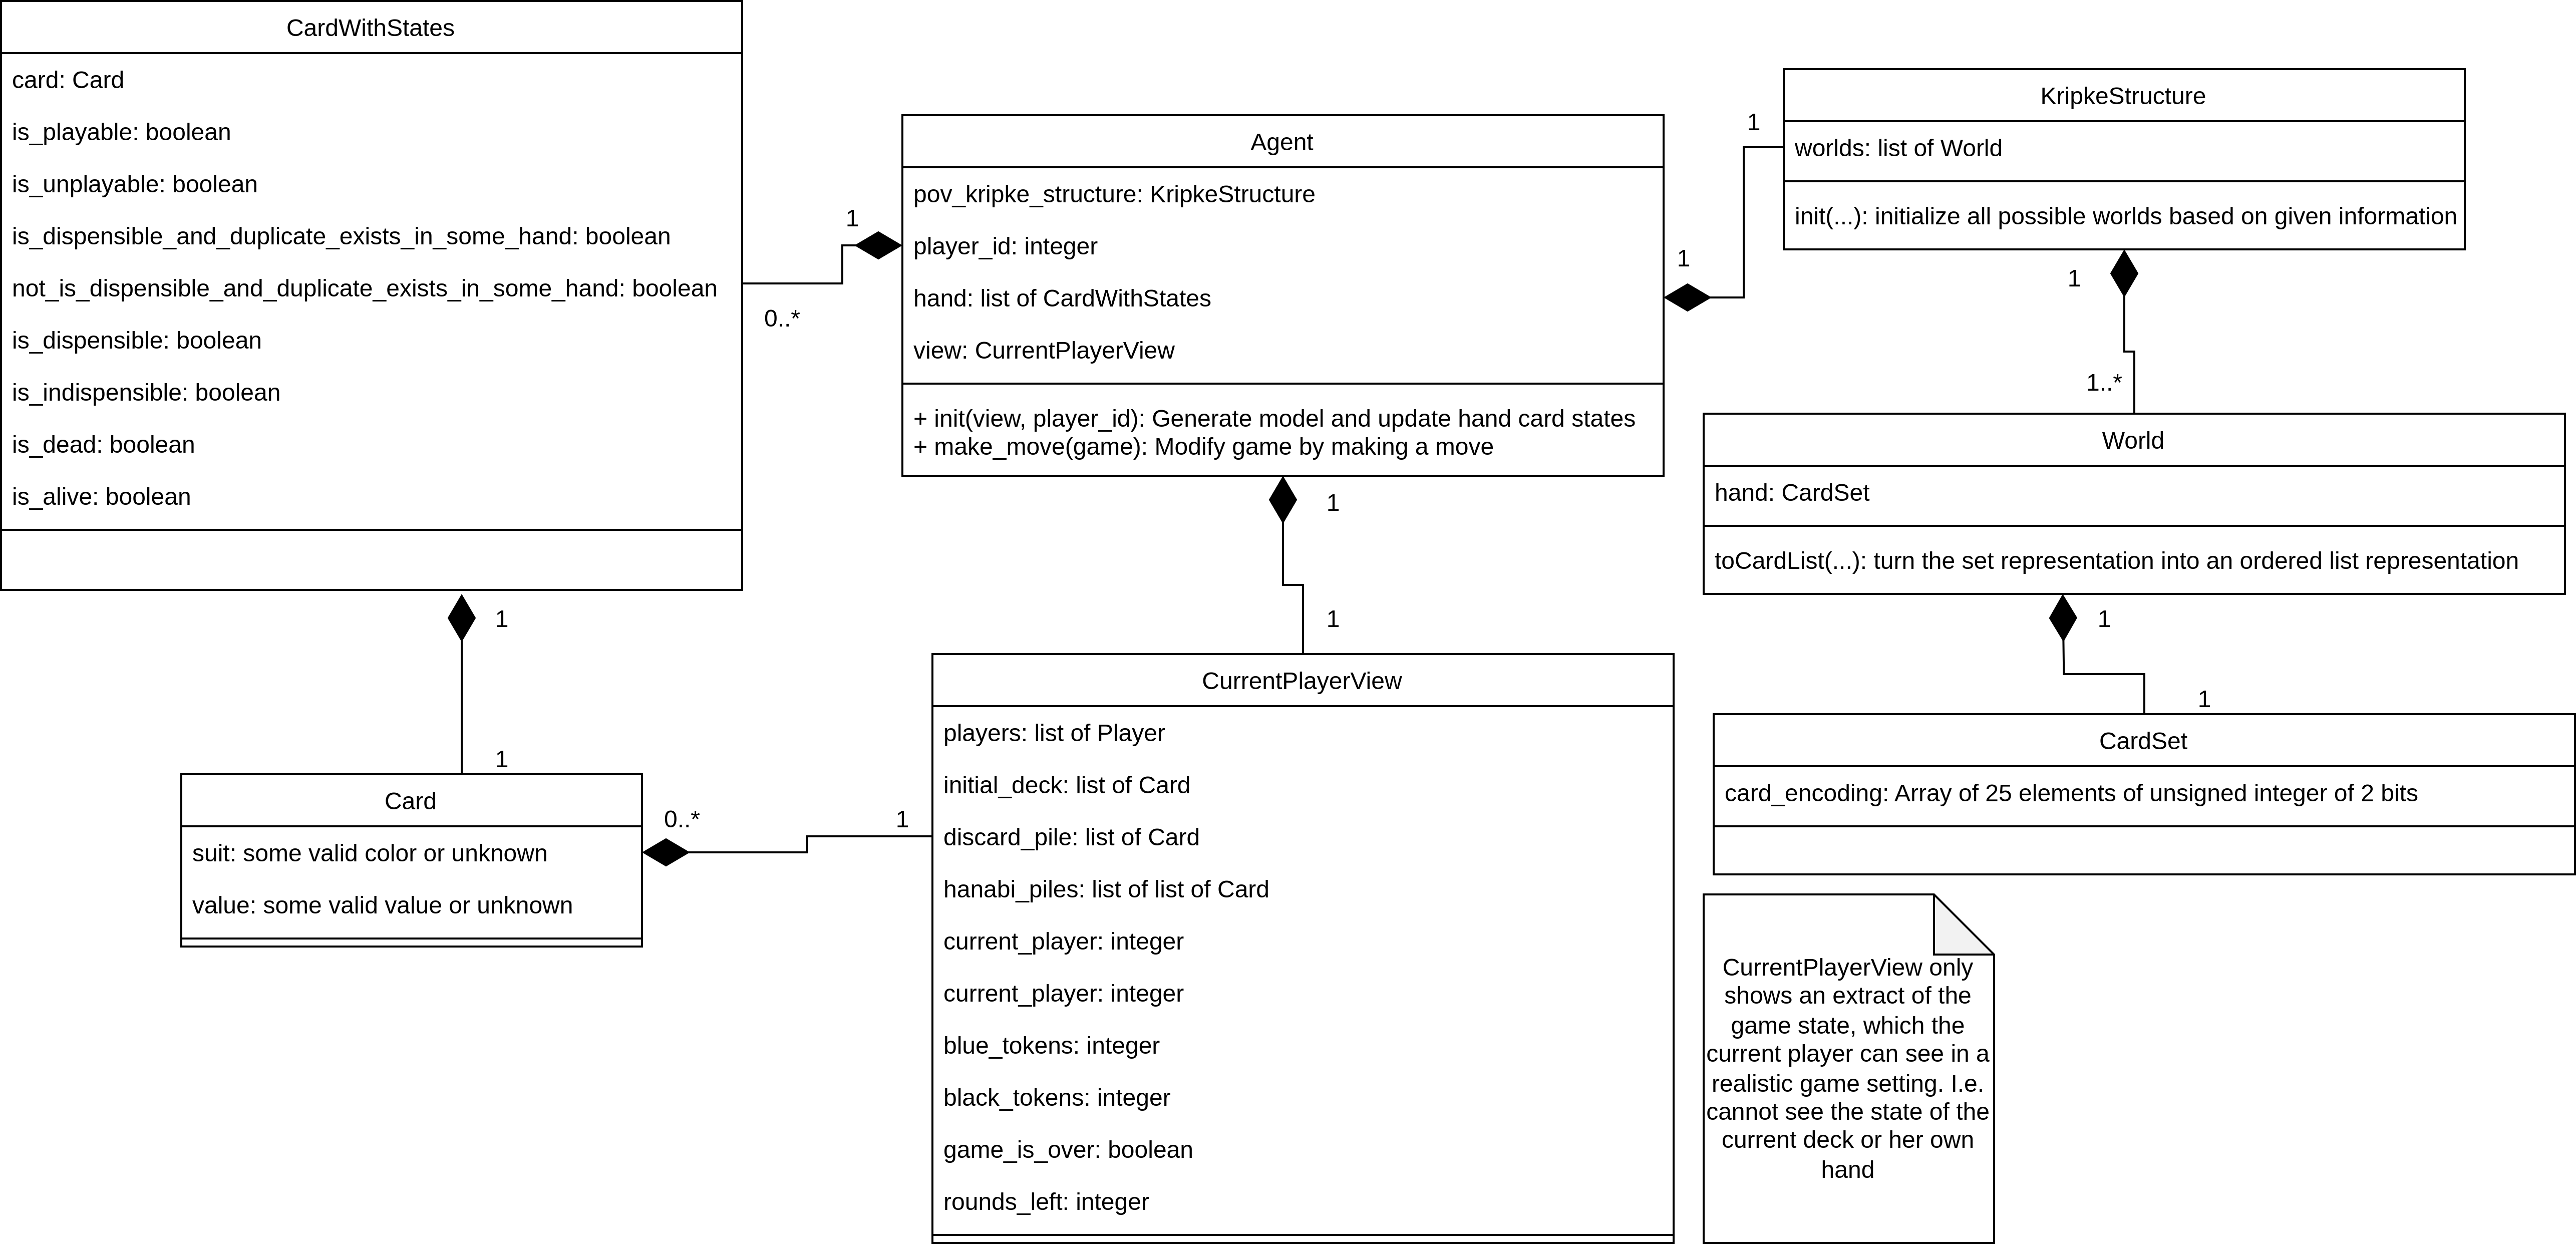
\includegraphics[width=22cm]{images/agent-uml-class-diagram.png}
	\caption{Low-fidelity class diagram for the things making up the Agent class}
	\label{fig:Agent-class-diagram}
\end{sidewaysfigure}

\subsection{Game simulation runner}
The glue-code between the {\tt Agent}s and the {\tt Game} classes, is a class called {\tt SimulationRunner} (defined in "{\tt src/ai\_simulation\_runner.zig}"), which takes a fully initialized Game and on-demand generates the agents and their epistemic models, and simulates a course of a game.
See Figure \ref{fig:SimulationRunner-class-diagram} for the components making up the game simulator.
The Game class has an element of randomness (in order to simulate random draws), so a seed can be provided when initializing the game in order to facilitate reproducibility.

\begin{figure}
	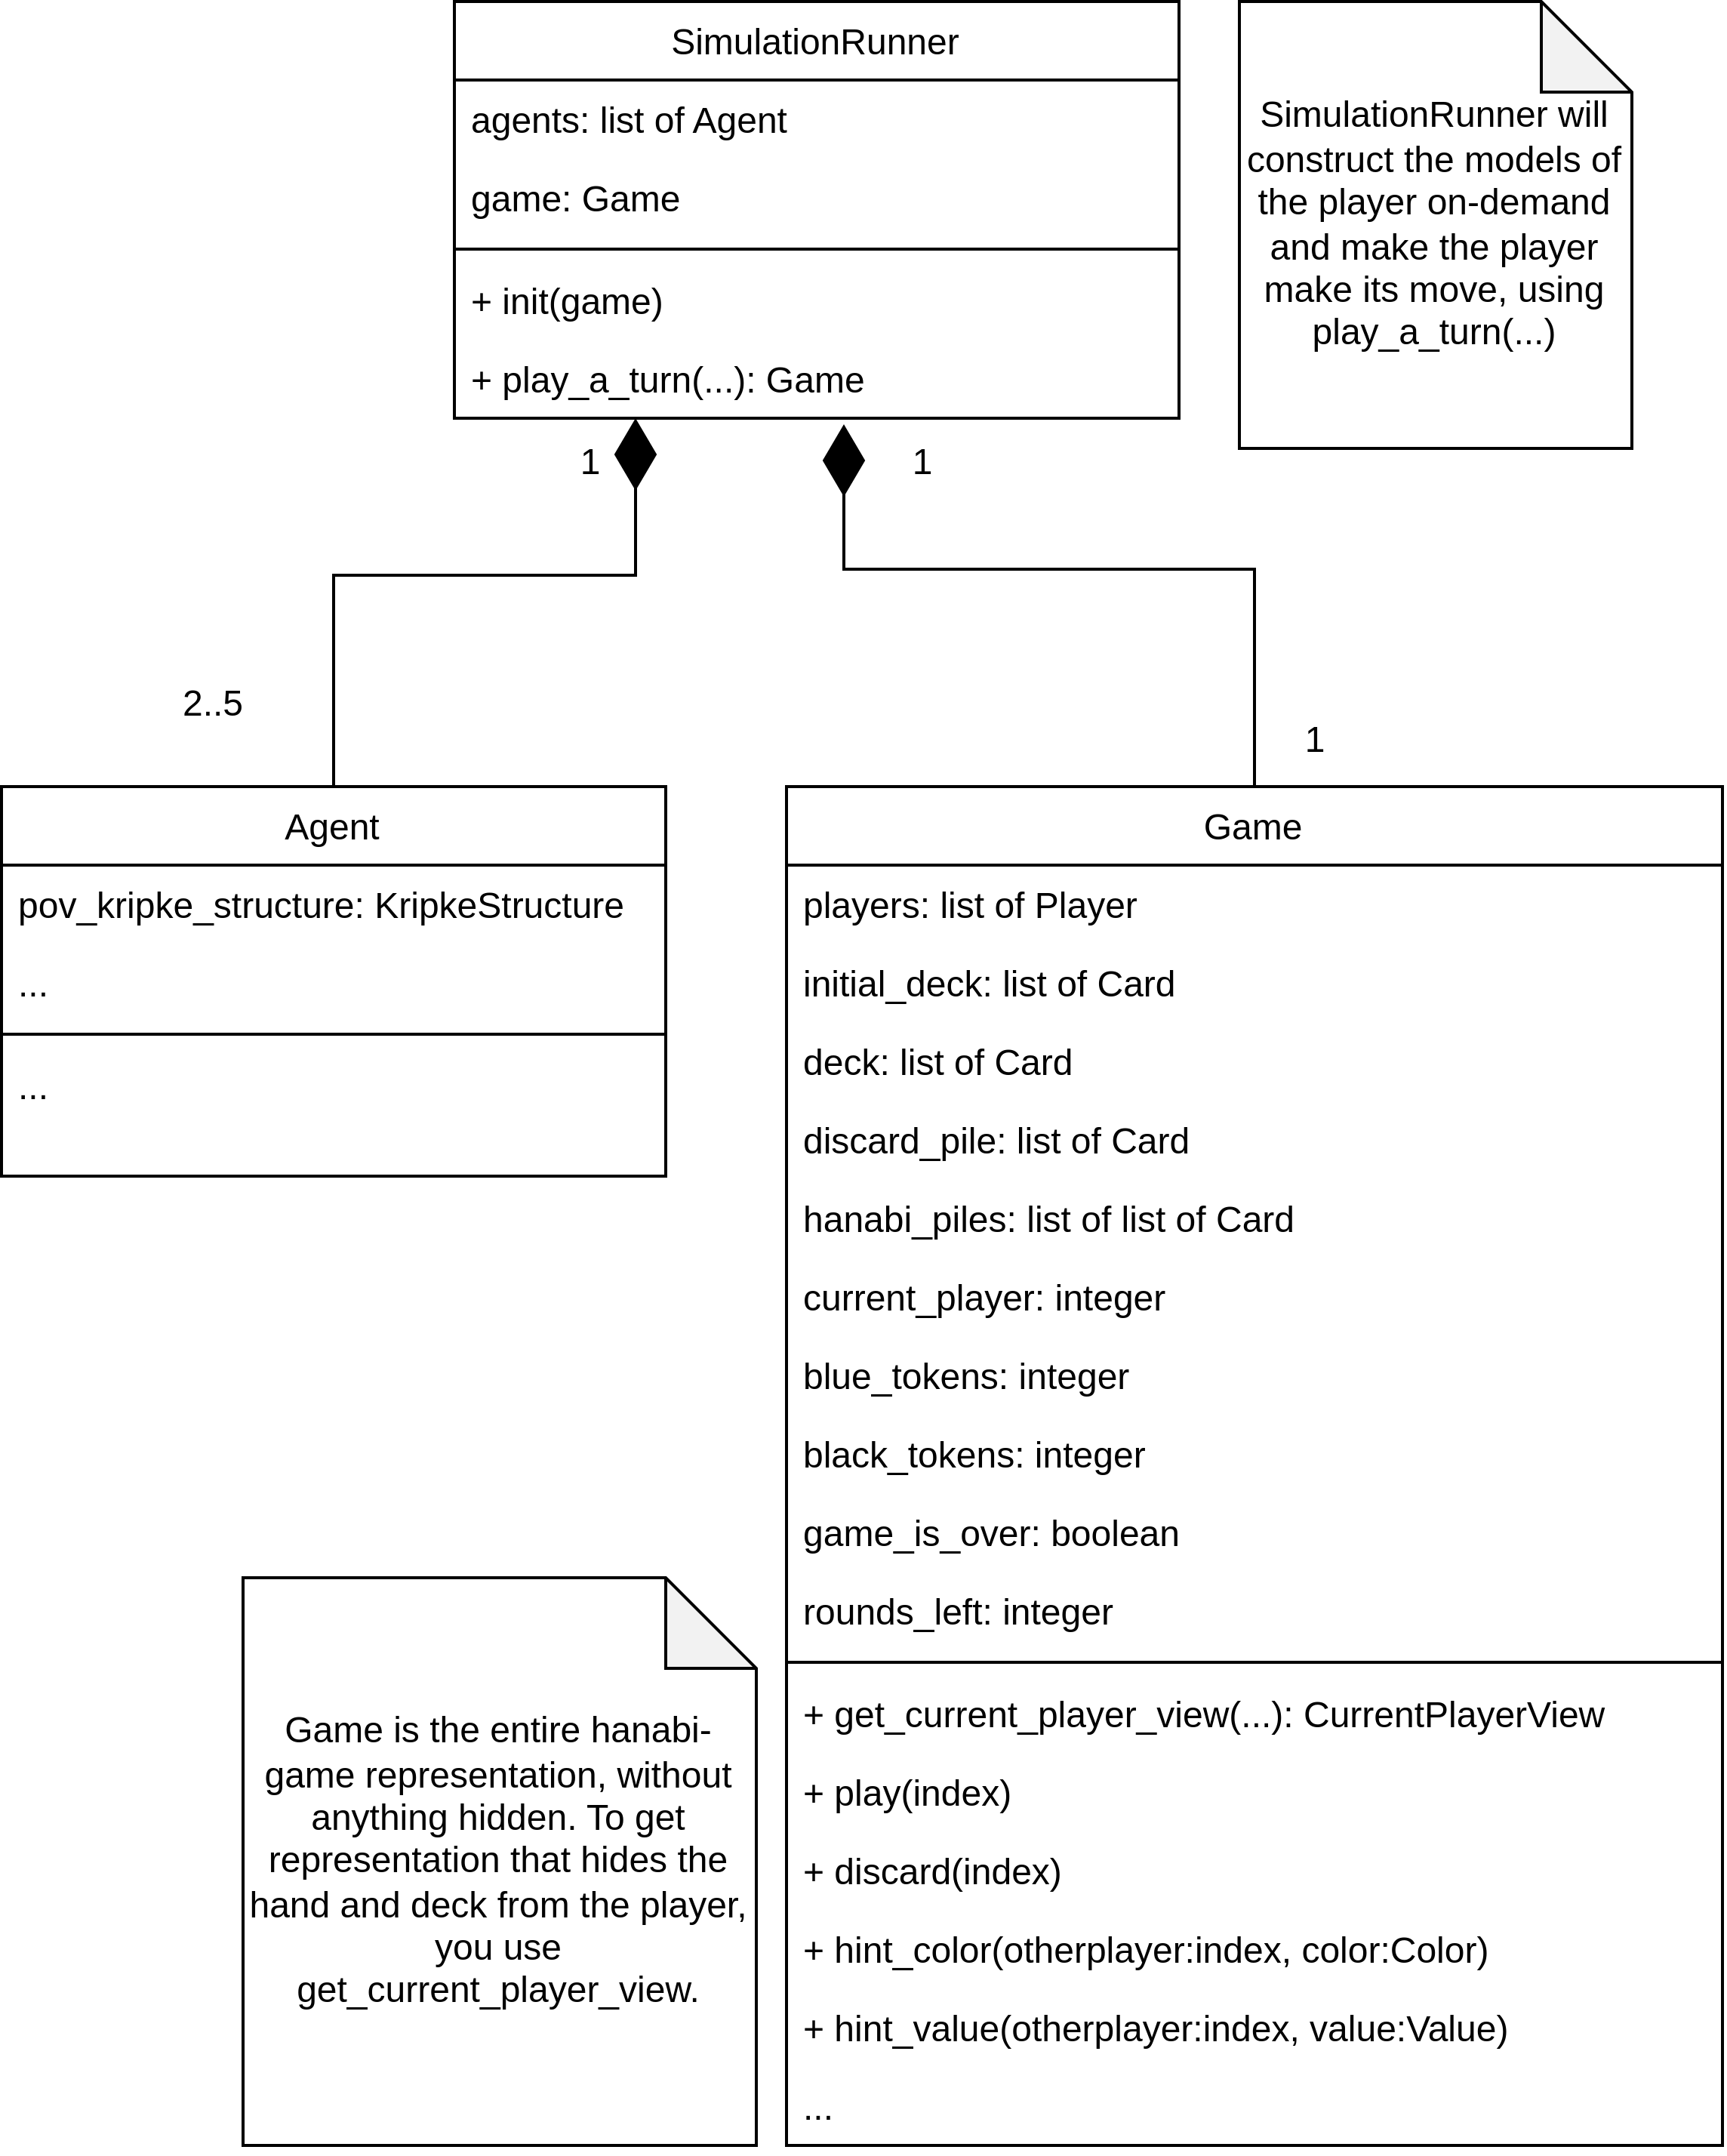
\includegraphics[width=13cm]{images/simulationrunner-uml-class-diagram.png}
	\caption{Low-fidelity class diagram for the things making up the SimulationRunner class}
	\label{fig:SimulationRunner-class-diagram}
\end{figure}
